\hspace{0.6 cm} Gravitational waves are produced by each and every body which is accelerating, for e.g. moving cars, air planes, humans, etc. However, they are too small to be noticed and detected with our current technology. In order to study gravitational waves, we need to look at object which are massive and much more bigger than our own solar system like black holes, neutron stars, or huge stars at the end of their lives like gamma ray bursts, pulsars, orbiting black holes, rapidly spinning neutron stars, etc. In fact our universe is filled with many such objects which produce gravitational waves with a significant amplitude and energy. This section was referred by \cite{Allen1996TheSG}, \cite{Neutron_wiki}, \cite{Linear}, \cite{sounds_of_space} \\

\noindent Gravitational wave sources have been divided into following categories:-

\begin{enumerate}
    \item \textbf{Short duration sources :-} Compact binary coalescence, supernovae, gamma ray burst.

    \item \textbf{Continuous sources :-} Pulsars, magnetars, rapidly spinning neutron stars, low mass X Ray binaries, super massive black hole binaries.

    \item \textbf{Stochastic sources :-} Metric fluctuations generated in the very early universe.
\end{enumerate}

\noindent To understand gravitational waves better, LIGO scientists have divided the waves in four categories. The division of the gravitational waves is based on their sources and their characteristic vibration as detected by the interferometers.  They are divided into Continuous, Compact Binary Inspiral, Stochastic and Burst Gravitational waves.

\begin{enumerate}

\item \textbf{Continuous Gravitational Waves} 
    
\noindent Such Gravitational Waves are produced by objects that have constant frequencies and amplitude like a single spinning neutron star. Neutron stars are basically a result of the supernova explosion of a massive star, combined with gravitational collapse, that compresses the core so much that the star density becomes as that of atomic nuclei. Radius of neutron stars will be in the order of 10 kilometers, and mass will be around 1.4 Solar masses. So density will be around $10^{17}\: \text{Kg}\text{m}^{-3}$. The properties of the gravitational waves depend on the spin rate of the star. Therefore, if the spin rate is constant, the properties of gravitational waves (frequency and amplitude) will also remain constant i.e. \textit{continuous}. Spinning neutron stars that possess asymmetric deformations or imperfections in their space produce gravitational waves as it swiftly rotates about its axis. The reasons or effects which can produce asymmetry could be Accretion (large mountain), Magnetic deformations or Pulsar glitches.

\vspace{0.2cm}

\item \textbf{Compact Binary Inspiral Gravitational Waves}
    
\noindent Most of the waves detected so far by LIGO are part of this category. Compact Binary In spiral Gravitational Waves are formed by orbiting pairs of massive objects like neutron stars or black holes. There are three kinds of systems in this category of gravitational wave generators where each one has different characteristics. They are Binary Black Hole system (BBH), Binary Neutron Star system (BNS) and Black Hole-Neutron Star binary system (BHNS). The main phases involved in such systems are spiral, merger and ring-down.

\vspace{1mm}
Let us start by considering two black holes orbiting each other. Initially they are widely separated, spiral occurs over millennia, with each revolution, they emit very weak gravitational waves. Slowly as the energy is lost from the system in the form of gravitational waves, the binary is thus pushed into an orbit with smaller radius and higher orbital frequency. Thus the distance between them decreases and their speeds increase. This causes the frequency of the gravitational waves to increase. Now comes the Merger stage where the black holes come very close and are about to collide to form a single black hole and the black hole thus formed has large distortions in its shape. The strongest gravitational waves are emitted during this process. The distortions thus formed are radiated away as more gravitational waves during the ring-down phase and an undistorted but rotating black hole is left behind. Due to the increase in frequency, the pitch also increases and as a result these gravitational waves would produce a chirp sound. Current results indicate that compact binary objects may well be the most promising sources of gravitational waves rather than supernova collapse.

\item \textbf{Stochastic Gravitational Waves}

These types of waves are generated from random sources, typically arising from a large number of unresolved and uncorrelated events and thus they are the most difficult gravitational waves to detect. Stochastic Gravitational Waves are believed to be the result of processes that took place shortly after the big bang. Just like the Cosmic Micro-wave Background (CMB), these gravitational waves arise from a large number of independent, random events merging to create a cosmic gravitational wave background. Due to their random motion, these waves are the most smallest, that's why the final signal has stochastic nature and the difficult to detect with our current technology. These waves may be analyzed statistically but they cannot be predicted precisely. Detecting these gravitational waves from the Big Bang could allow us to see back in the history of the Universe.

\vspace{0.2cm}

\item \textbf{Burst Gravitational Waves}   

Of all the types of gravitational waves, these waves come from the sources which are yet to be known and thus the form of waves which will be produced is also unexpected. Burst gravitational waves come from short-duration unknown sources. Since we are unfamiliar with these sources, thus its modelling is a big challenge since these will not have well defined properties which are known earlier to us like those of compact binary inspiral waves. Some believe that these waves are produced from systems like supernovae. They are believed to have a 'pop' and 'crack' sound. However, it is difficult to say anything as of now due to the lack of knowledge about their origin. But if we discover an efficient way to detect such GW, revolutionary information about the universe could be revealed.

\end{enumerate}

\begin{figure}[h]
    \centering
    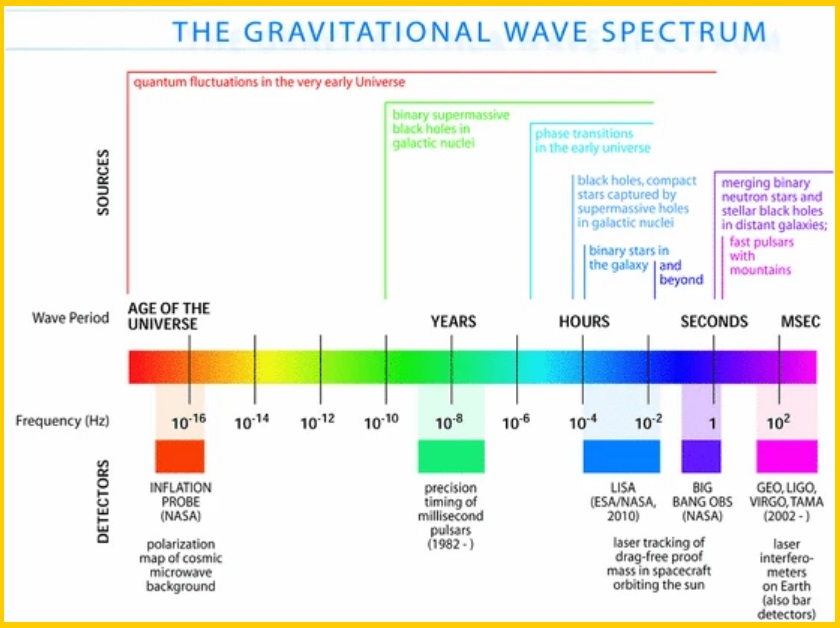
\includegraphics[scale=0.6]{images.tex/Stochastic_gw.jpg}
    \caption{Gravitational Wave Spectrum. Source :- \href{https://link.springer.com/article/10.1007/s41114-017-0004-1}{Detection methods for stochastic gravitational-wave backgrounds by Joseph D. Romano}}
\end{figure}

\begin{figure}[h]
    \centering
    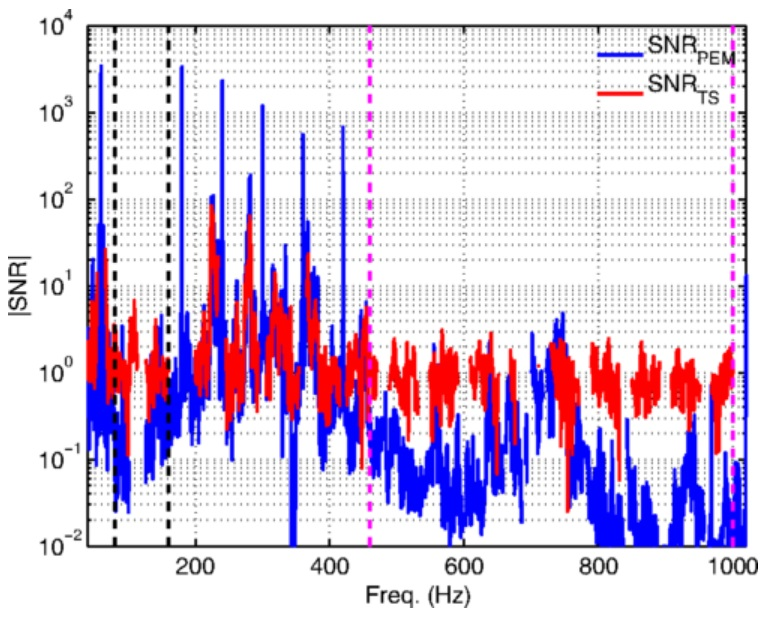
\includegraphics[height = 3.5 cm, width = 10cm]{images.tex/Stochastic wave form.jpg}
    \caption{Stochastic gravitational wave form.\, Source :- \href{https://journals.aps.org/prd/abstract/10.1103/PhysRevD.91.022003}{Searching for stochastic gravitational waves using data from the two co-located LIGO Hanford detectors by J. Aasi}}
\end{figure}

\pagebreak



















































\pagebreak